                                                                                                                                                                                                                                                                                                                                                                                                                            \documentclass[11pt]{beamer}
\usepackage{setspace}
\usepackage{graphicx} % insert pdfs
\usepackage{sansmathaccent}
\pdfmapfile{+sansmathaccent.map}

\usetheme{Warsaw}


\title{Grid Search Pipeline for Mean Reversion Time Series}
\subtitle{}
\author{Peixin (Elvin) Ning}
\institute{\normalsize{peixin.ning@hotmail.com}}
\date{March 19 Tuesday, 2019}
\begin{document}

	
\begin{frame}
\titlepage
\end{frame}

\begin{frame}
\frametitle{Roadmap}
\begin{spacing}{1.5}
	\begin{itemize}
	\item Generate data with O-U process
	\item Mean reversion test 
	\item Crossed limit trigger (Gaussian deviation)
	\item Time to mean revert and half life
	\item Trades and metrics
	\item Grid search framework
\end{itemize}
\end{spacing}

\end{frame}


\section*{Generate data with O-U process}
\subsection*{O-U process}

\begin{frame}
\frametitle{Definition and properties of O-U process}
When it comes to mean reversion, a classic stochastic process in probability theory is the Ornstein--Uhlenbeck process $\{X_t\}_{t \geq 0}$ defined by the following stochastic differential equation{:}
\begin{center}
	 $dX_t =\theta (\mu - X_t)dt + \sigma dW_t$
\end{center}
Property:
	\begin{itemize}
	\item Stationary, Gaussian, and Markovian.
	\item {\bf Mean-reverting} towards the long-term mean $\mu$ with "speed" $\theta$.
	\item  Continuous-time analogue of the discrete-time AR(1) process
	$X_t = c + \lambda X_{t-1} +\epsilon_t$
	\end{itemize}
\end{frame}

\subsection*{Data generation}
\begin{frame}
\frametitle{Euler-Maruyama approximation to the process}
Assuming the following approximation:
	\begin{center}
		$dt \approx  t_{n+1}-t_n$
		
		$dW_t \approx W_{t_{n+1}} - W_{t_{n}}$
	\end{center}
and recursively define:
	\begin{center}
	$X_{n+1}=X_n + \theta (\mu - X_n) +\sigma(W_{t_{n+1}} - W_{t_{n}})$
	\end{center}
	where increment step $dt$ is sufficiently small.
\end{frame}

\begin{frame}
\frametitle{Data series generated by O-U}
\noindent\makebox[\textwidth]{\includegraphics[width=\paperwidth]{../images/series.pdf}}
\end{frame}

\section*{Statistical test of mean reversion}
\subsection*{Augmented Dickey--Fuller test}
\begin{frame}
\frametitle{Augmented Dickey-Fuller test}
Given a time series model
\begin{center}
$\Delta X_t=\alpha+\beta t +\lambda X_{t-1} +\delta_1\Delta X_{t-1} + \cdots +\epsilon_t$
\end{center}
test null hypothesis $H_0:\lambda=0$ vs. $H_A:\lambda<0$, with test statistic:
\begin{center}
	$DF=\frac{\hat{\lambda}}{SE(\hat{\lambda})}$
\end{center}
If $DF$ is less than the critical value, then the null hypothesis of $\lambda=0$ is rejected and no unit root is present.
\end{frame}

\begin{frame}[fragile]
\frametitle{Augmented Dickey-Fuller test}
\begin{verbatim}
statsmodels.tsa.stattools.adfuller(X[:250*24])

(-6.0785694575222715,
1.106265283568116e-07,
2,
5997,
{'1%': -3.4314408956603097,
'5%': -2.8620220755599486,
'10%': -2.5670266063699962},
-49313.968981484046)
\end{verbatim}
The first and second outputs are test statistic and p-value. We reject the hypothesis of unit root. The series is indeed mean reverting. (Since we generate it using a mean reverting stochastic process.)
\end{frame}

\subsection*{Alternative approaches}
\begin{frame}
\frametitle{Hurst exponent and other unit root test}
Other unit root test for stationarity:
\begin{itemize}
	\item Hurst exponent for mean reverting vs. trending
	\item Kwiatkowski-Phillips-Schmidt-Shin (KPSS) tests
	\item Phillips-Perron test (PP)
	\item ADF-GLS test procedure (ERS) 
\end{itemize}
\end{frame}



\section*{Crossing limit}
\subsection*{Price deviation and Gaussion detection}
\begin{frame}
\frametitle{Price deviation signal}
Given the generated time series $X_t$, if the current price $x$ is very far from the long-term mean $\mu$, we detect the signal of crossing limit.

For simplicity, we use Gaussian model for detection of large deviation. 

First, we estimate the MLE for mean and deviation.
\begin{center}
	$\hat{\mu}= \frac{1}{M}\sum_{i=1}^{M}X_i$
	
	$\hat{\sigma} = \sqrt{\frac{1}{M}\sum_{i=1}^{M}(X_i-\hat{\mu})^2}$

\end{center}
Note the standard deviation is biased estimator, but it doesn't really matter in our case.
\end{frame}

\begin{frame}
\frametitle{Gaussian anomaly detection}
Our series is generated by O-U process, with a lot of "good properties". The histogram is:
\begin{center}
	\noindent\includegraphics[scale=0.45]{../images/hist.pdf}
\end{center}
The Gaussian anomaly detection model works remarkably well. 
\end{frame}


\subsection*{Probability level to determine crossing limit}
\begin{frame}[fragile]
\frametitle{Inverse given a probability level $p$}
If we specify the one-side probability $p$ of how rare the crossing event happens, we calculate the inverse based on the model as the crossing limit.
\begin{verbatim}
level = [0, 0.01, 0.05, 0.1, 0.3, 
	0.5, 0.7, 0.9, 0.95, 0.99, 1]
inv = stats.norm.ppf(level, mu_MLE, sigma_MLE)
\end{verbatim}
This is a hyperpamameter to determine the crossing limit.
\end{frame}

\begin{frame}
\frametitle{Exiting limit}
A natural way to determine the exit is to specify the probability of how much the series returns to normality, namely the long-term equilibrium mean $\mu$. 

This hyperparameter, probability level, can be combined with a classic time hyperparameter, the half life, as we introduce in the next section.
\end{frame}

\section*{Time to mean revert}
\subsection*{Half life}
\begin{frame}
\frametitle{Half life}
The half life is originated from nuclear physics and highly related to the O-U process:
\begin{center}
	$dX_t =\theta (\mu - X_t)dt + \sigma dW_t$
\end{center}
The half life of an O-U process is define as:
\begin{center}
$hl=\frac{ln(2)}{\theta}$
\end{center}
\end{frame}

\subsection*{Estimation of half life}
\begin{frame}[fragile]
\frametitle{Estimation of half life}
As we mentioned early, the mean-reverting process can be discretized to an AR process:

\begin{center}
	$\Delta X_t = -\theta X_{t-1} \Delta t +\epsilon_t$
\end{center}
 We can regress $X_t$ against $X_{t-1}\Delta t$ in a linear model and estimate $\theta$.
\begin{verbatim}
granularity = 1
xx = X_train[1:-1].reshape((m, 1)) 
yy = (np.roll(X_train, -granularity)[1:-1] 
- X_train[1:-1]).reshape((m, 1)) 

reg = LinearRegression().fit(xx, yy)
\end{verbatim}
\end{frame}

\begin{frame}[fragile]
\frametitle{Plot of linear mean reverting coefficient}
Note that the slope is negative here suggests $\theta > 0$ (Coefficent $<0$), which implies the mean reverting property.
\begin{center}
	\noindent\includegraphics[scale=0.4]{../images/linreg.pdf}
\end{center}

\begin{verbatim}
hl = np.asscalar(- np.log(2) / reg.coef_)
Half life is 58.952675 * 1.000000 hours
\end{verbatim}

\end{frame}

\subsection*{Hyperparamters}
\begin{frame}
\frametitle{Half life and time step $\Delta t$ as hyperparamters}
Half life provides a good guidance about how long the series pull back half to the mean. Our pairs hyperparameters  can be set as multiples of $hl$, depending on $\Delta t$. For instance:
\begin{center}
	$M = [0.5hl, 0.75hl, hl, 1.25hl, 1.5hl, 2hl]$
	
	$\Delta t = [1, 2, 12, 24]$
\end{center}
\end{frame}

\section*{Trades, profit and grid search}
\subsection*{Make trades based on probability level $p$ and $hl$}
\begin{frame}[fragile]
\frametitle{Return $Y\%$ based on entry and half life}
Given $p1=0.05$,
\begin{verbatim}
entry = (stats.norm.ppf(p1, mu_MLE, sigma_MLE), 
stats.norm.ppf(1 - p1, mu_MLE, sigma_MLE))
\end{verbatim}

Given "normal" $p2=0.3$ or estimated half life 
\begin{center}
$(hl,\Delta t)=(59,1)$
\end{center}
determine the reverted price level and the "at least Y\% return" in our problem, where 
\begin{center}
	$Y\% = \frac{new price level - entry}{entry}$
\end{center}

\end{frame}

\subsection*{Calculate profit}

\begin{frame}[fragile]
\frametitle{Calculate profit}
\begin{verbatim}
trades = np.empty((0,3)) # [entry, exit, long or short]

profit = (trades[:-1, 1] - trades[:-1, 0]) * trades[:-1, 2]
sum(profit)

profit is 5.476257671422052
\end{verbatim}

For each tuple of parameters $(p, hl_{\Delta t}, \Delta t)$, we have a correspondent profit. This motivates a grid-search framework as follows:
\end{frame}

\subsection*{Grid search pipeline}
\frametitle{Grid search}
\begin{frame}
Pseudo Code for grid search:
\begin{itemize}
	\item For $p1$ in $[0.05, 0.1, 0.2]$, get crossing limit X.
	\item For $dt$ in $[1, 2, 12, 24, ...]$, get half life $hl$.
	\item For period in $[0.5, 0.75, 1, 1.5, 2, ...]*hl$, combined with $p2$, get return $Y\%$.
	\item Combine X, Y and periods, make trades and calculate profit (or other metrics).
	\item Maximize $profit(p, dt, hl)$ = maximize $profit(X,Y, M, N)$ in our problem.
\end{itemize}
\end{frame}

\section*{Further improvement}
\begin{frame}
\frametitle{Possible improvements}
\begin{itemize}
	\item More realistic data.
	\item With more samples and better data quality, we can use signals as simply as Bollinger bands, or as advanced as neural network, support vector machine or random forest to get the optimal crossing limit $X$.
	\item No stop loss in our trades.
	\item More metrics such as sharpe ratio and drawdown.
\end{itemize}
\end{frame}

\begin{frame}
\frametitle{SVM classifier example}
Below is novelty detection of 2-dimensional data using support vector machine.
\begin{center}
	\noindent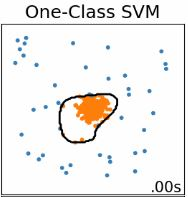
\includegraphics[scale=0.7]{../images/svm.jpg}
\end{center}
For realistic asset, we can train the data with many meaningful features and set the decision boundary as the "crossed limit".

\end{frame}


\begin{frame}
\frametitle{References}
[1] An Algorithmic Introduction to Numerical Solution of Stochastic Differential Equations, Desmond J. Higham.

[2] Algorithmic Trading: Winning Strategies and Their Rationale, Ernie Chan.

[3] Andrew Ng's Machine Learning Course: Anomaly Detection.

[4] Time Series: Theory and Methods, Peter J. Brockwell \& Richard A. Davis.

\end{frame}

\end{document}